\chapter{Power Amplifier Imperfections}\label{ch:1}

\section{Amplifier non-linearity}

\begin{figure}[H]
\centering 
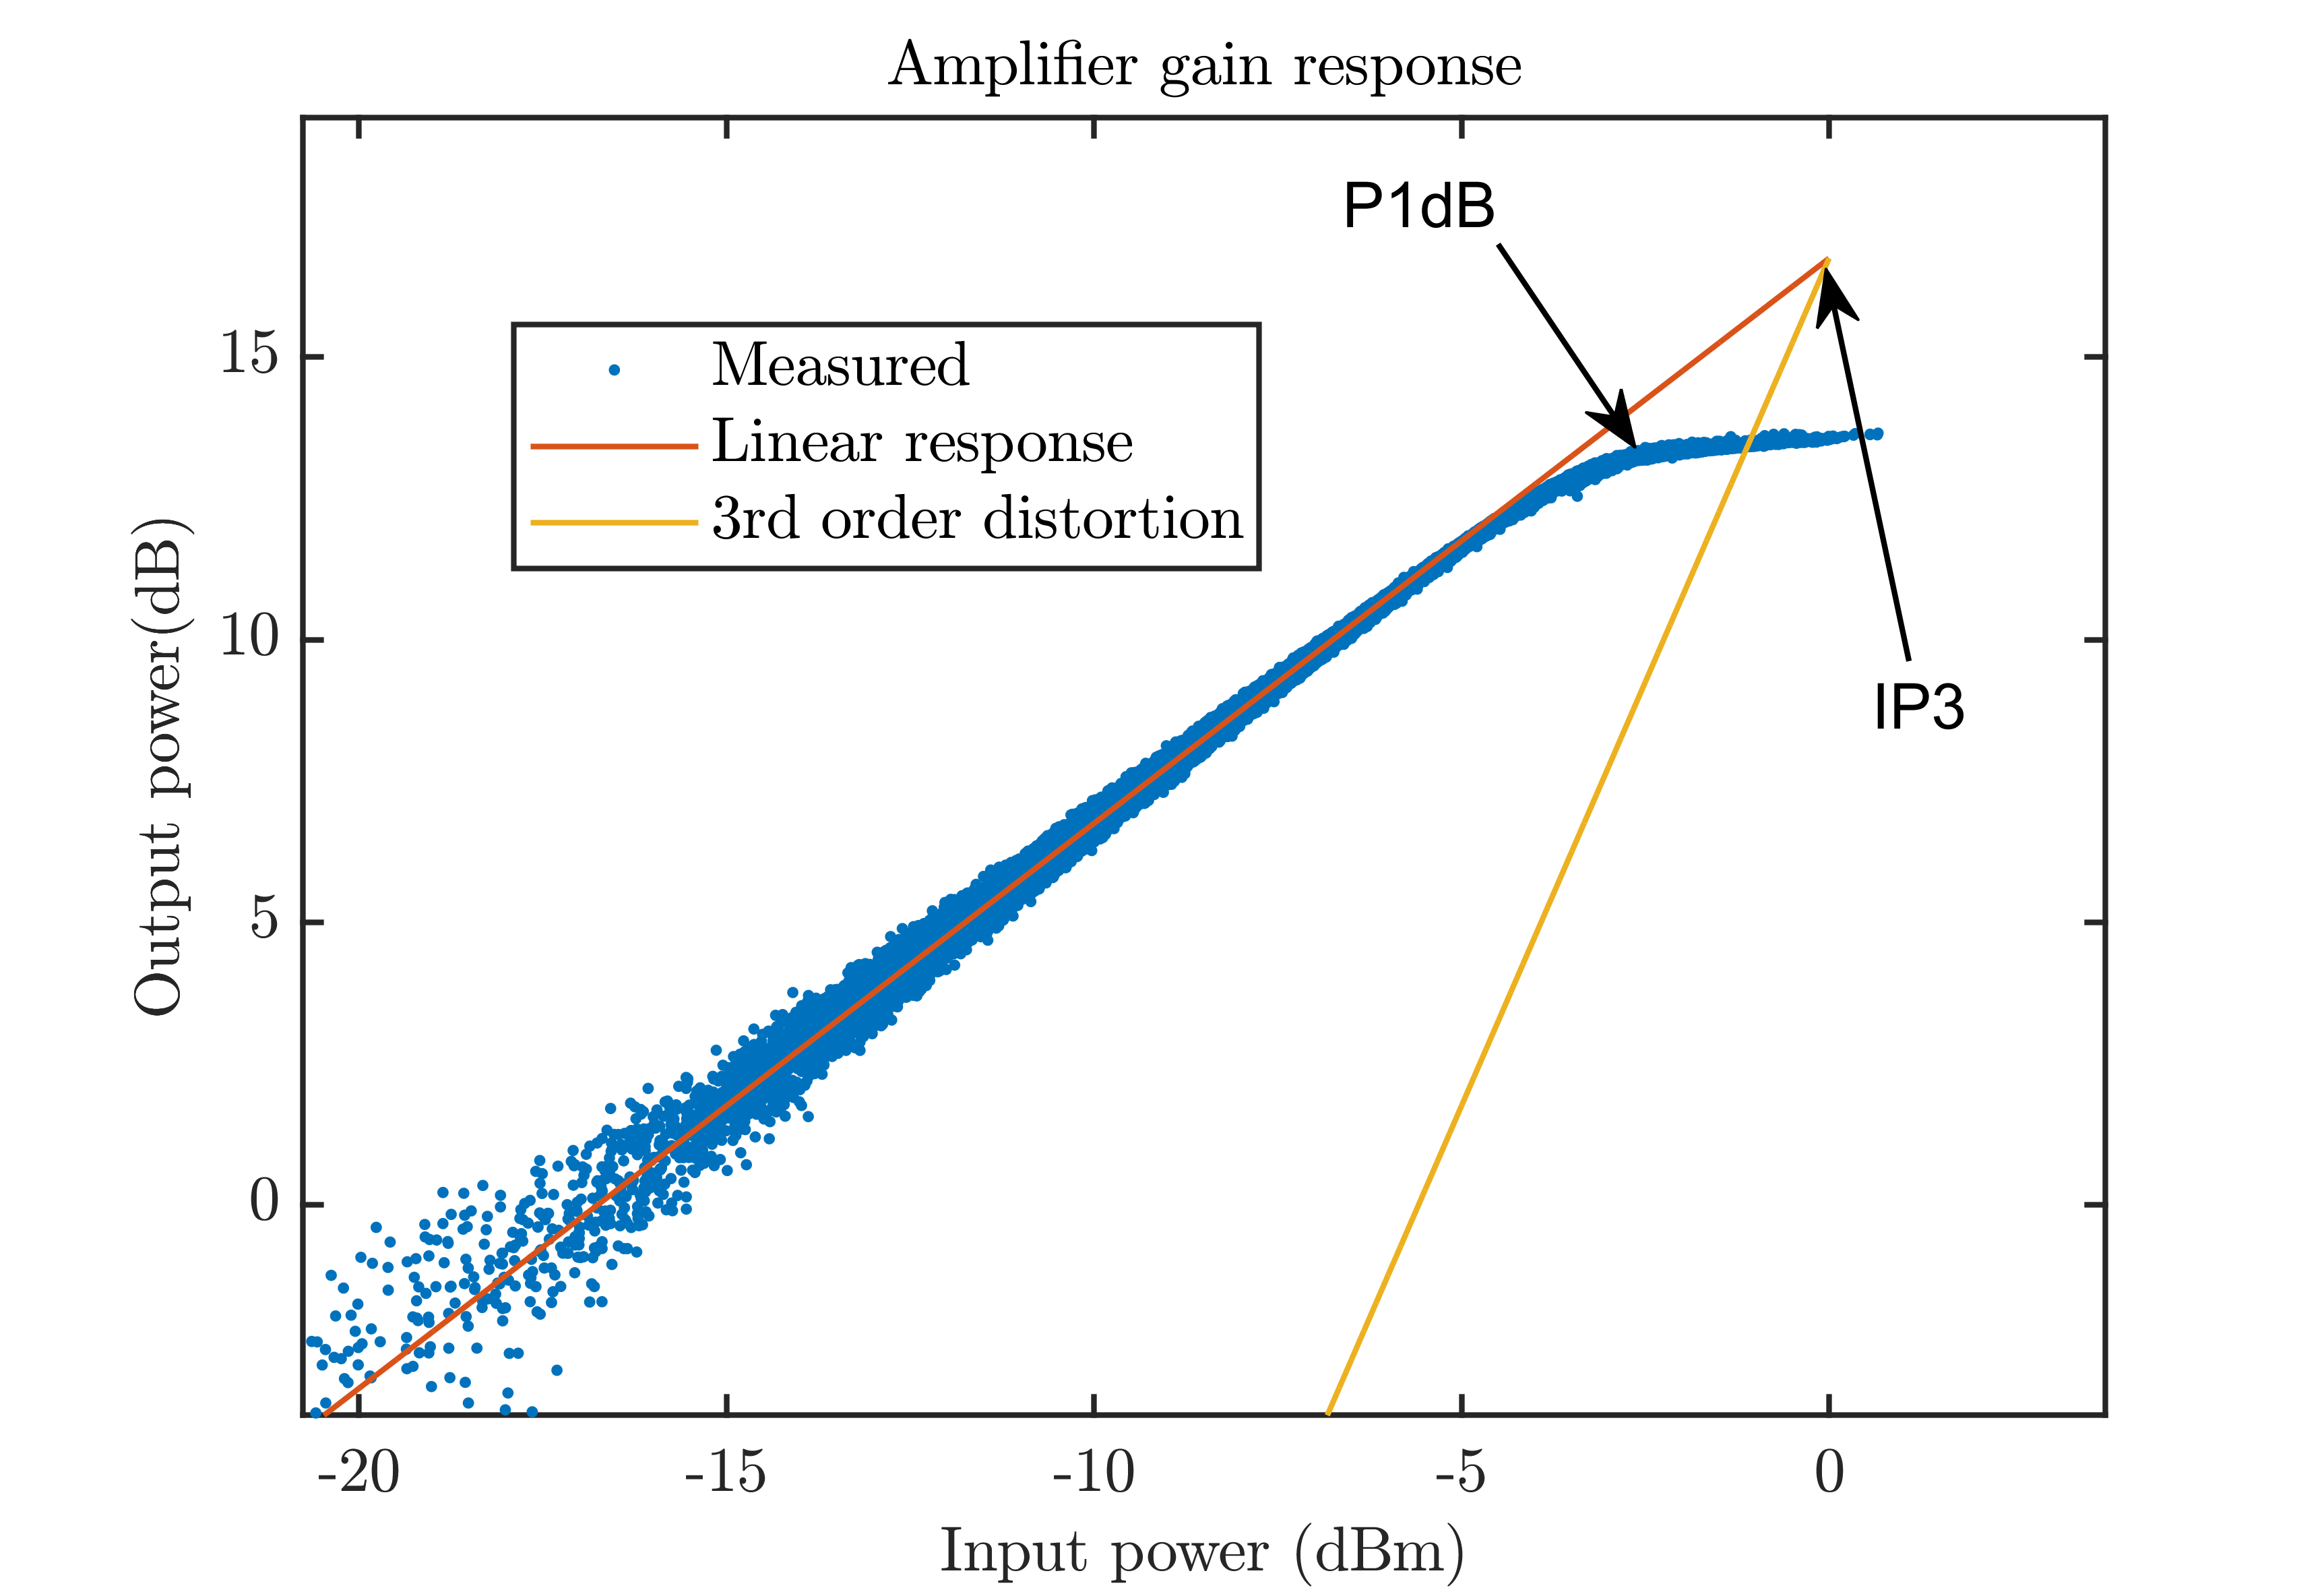
\includegraphics[scale = 0.4]{figures/ch1/amp_lin.png}
\caption{Amplifier non-linearity \citep{NI}}
\label{fig:amp_lin}
\end{figure} 

A power amplifier (PA) has a voltage-in to voltage-out relationship that can be described by the figure depicted in \ref{fig:amp_lin} as actual fundamental response. This causes a distortion at the output which can be described by equation \ref{eq:dest} \citep{NI}. 

\begin{equation} \label{eq:dest}
V_{out} = a_0 + a_1 V_{in} + a_2 V_{in}^2 + a_3 V_{in}^3 + a_4 V_{in}^4 + ... 
\end{equation}

Where $V_{out}$ is the output signal from the amplifier, $a_1, a_2 ,a_3..$ is coefficients describing the ratio of the distortion and $V_{in}$ is the input. If a single tone input is presented, then the output will consist of purely odd and even harmonic distortion. If a input-signal using two tones is considered then there will be a difference and a sum of the frequencies presented at the output which is caused by the cubic term in equation \ref{eq:dest2}. This is also called Two-Tone Third-Order Intermodulation Distortion and is also depicted in figure \ref{fig:amp_lin} as 3rd order distortion with a slope of 3:1. It can bee seen that when the output power increases then the distortion increases 3 times. A measurement of this is called the third-order-intercept-point (IP3 or TOI). However, the intersection is fictitious it is realized only in
mathematics and used as a figure of merit in industry. It can bee seen from figure \ref{fig:amp_psd} that the distorted component are spaced too close in frequency to be effectively filtered, which would need an other technique to be removed. Such a technique could be Digital Pre-Distortion (DPD)  

\begin{equation}\label{eq:dest1}
V_{in} = sin(\omega_1 t) + sin(\omega_2 t)
\end{equation} 

\begin{equation} \label{eq:dest2}
V_{out} = a_0 + a_1 (sin(\omega_1 t) + sin(\omega_2 t)) + a_2 (sin(\omega_1 t) + sin(\omega_2 t))^2 + a_3 (sin(\omega_1 t) + sin(\omega_2 t))^3 + ... 
\end{equation}


\begin{figure}[H]
\centering 
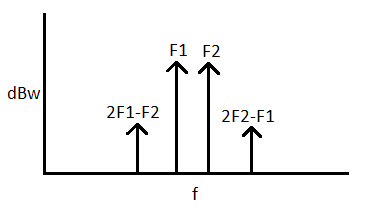
\includegraphics[scale = 0.7]{figures/ch1/amp_psd.png}
\caption{Two-Tone Third-Order Intermodulation Distortion}
\label{fig:amp_psd}
\end{figure}

\begin{figure}[H]
\centering 
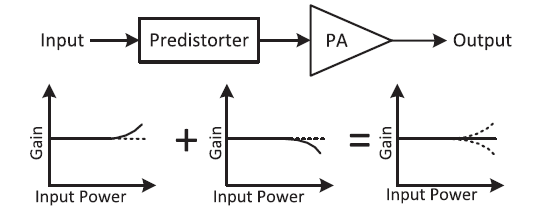
\includegraphics[scale = 0.7]{figures/ch1/predistortion_consept.png}
\caption{Consept of predistortion \citep{guo2015}}
\label{fig:pre_cons}
\end{figure}

In figure \ref{fig:pre_cons} the consept of DPD is depicted. DPD is a way to "distort" the incomming signal with the inverse transfer-function of the amplifier. For example the gain of the amplifier is ideally linear in the small-signal region and gets non-linear at higher signal levels. To overcome this, a block called the predistorter inverses this non-linear curve which is the exact inverse of the PA, then a linear amplification can be achieved at the final PA output. But to archive this exat inverse of the PA all the non-linear effects has to be accounted for.   

\subsection{Impact of non-linearity}
\begin{figure}[H]
\centering 
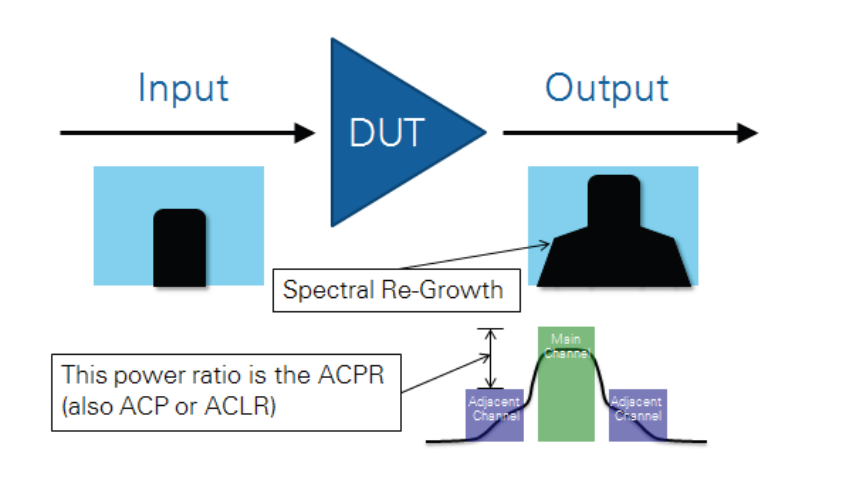
\includegraphics[scale = 0.5]{figures/ch1/acpr.png}
\caption{Graphical Depiction of ACPR in the frequency domain \citep{NI}}
\label{fig:acpr}
\end{figure}

Due to the imperfections of the PA spectral regrowth will occur which will affect nearby channels. The Adjacent Channel Power Ratio (ACPR) is a measure of the power of the distortion components, caused by the non-linearity of the PA, that are leaked into the adjacent channel see figure \ref{fig:acpr}. The formula for the ACPR is given by equation \ref{eq:acpr} and is used after a Fourier transform has been performed at the output of the PA.

\begin{equation} \label{eq:acpr}
	ACPR = \frac{\int_{adjch}^{} |Y(f)|^2 df }{\int_{mainch}^{} |Y(f)|^2 df}
\end{equation}   

Where $Y(f)$ is the Fourier transform of the signal, adjch is the adjacent-channel and mainch is the main-channel. 

\begin{figure}[H]
\centering 
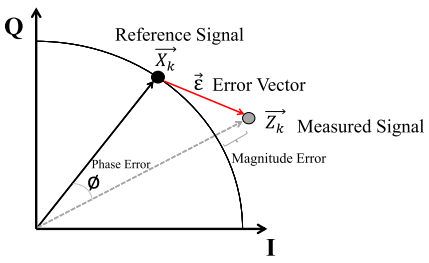
\includegraphics[scale = 0.8]{figures/ch1/evm.png}
\caption{Graphical view of the EVM}
\label{fig:evm}
\end{figure}
  
Another measure of the error is the Error Vector Measurement (EVM) or  Relative Constellation Error (RCE) which both is a measure of the error due to the constellations points in a IQ plot. If a signal is sent through an amplifier with a given IQ value, then the amplifier will distort those IQ values. The EVM and RCE is a measure of the power of the error vector divided by the power of the reference vector. \citep{ali2016}

\begin{equation} \label{eq:evm}
	EVM = \frac{P_{error}}{P_{reference}} = \frac{E[|z(t)-x(t)|^2]}{E[|x(t)^2|]}
\end{equation}  
 
\begin{figure}[H]
\centering 
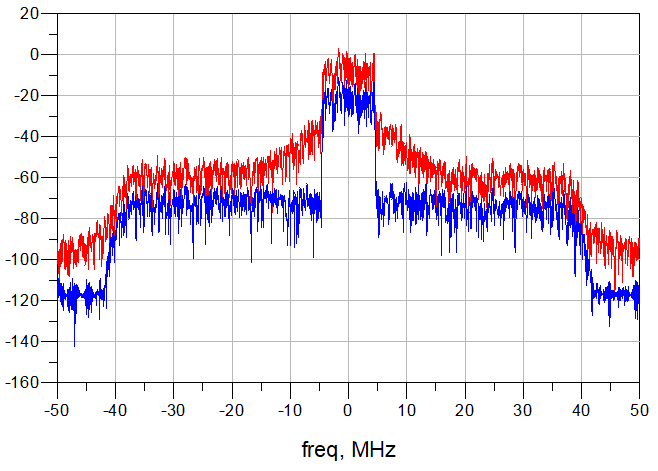
\includegraphics[scale = 0.5]{figures/ch1/ads_nonlin_dest.png}
\caption{Destortion simulated in ADS, where blue is input-signal and red is output-signal. The simulation is made with a single amplifier connected to a $50\Omega$ resistor. It is clearly that the output-signal is distorted.}
\label{fig:pre_cons}
\end{figure}

\section{Memory effects}

\begin{figure}[H]
\centering 
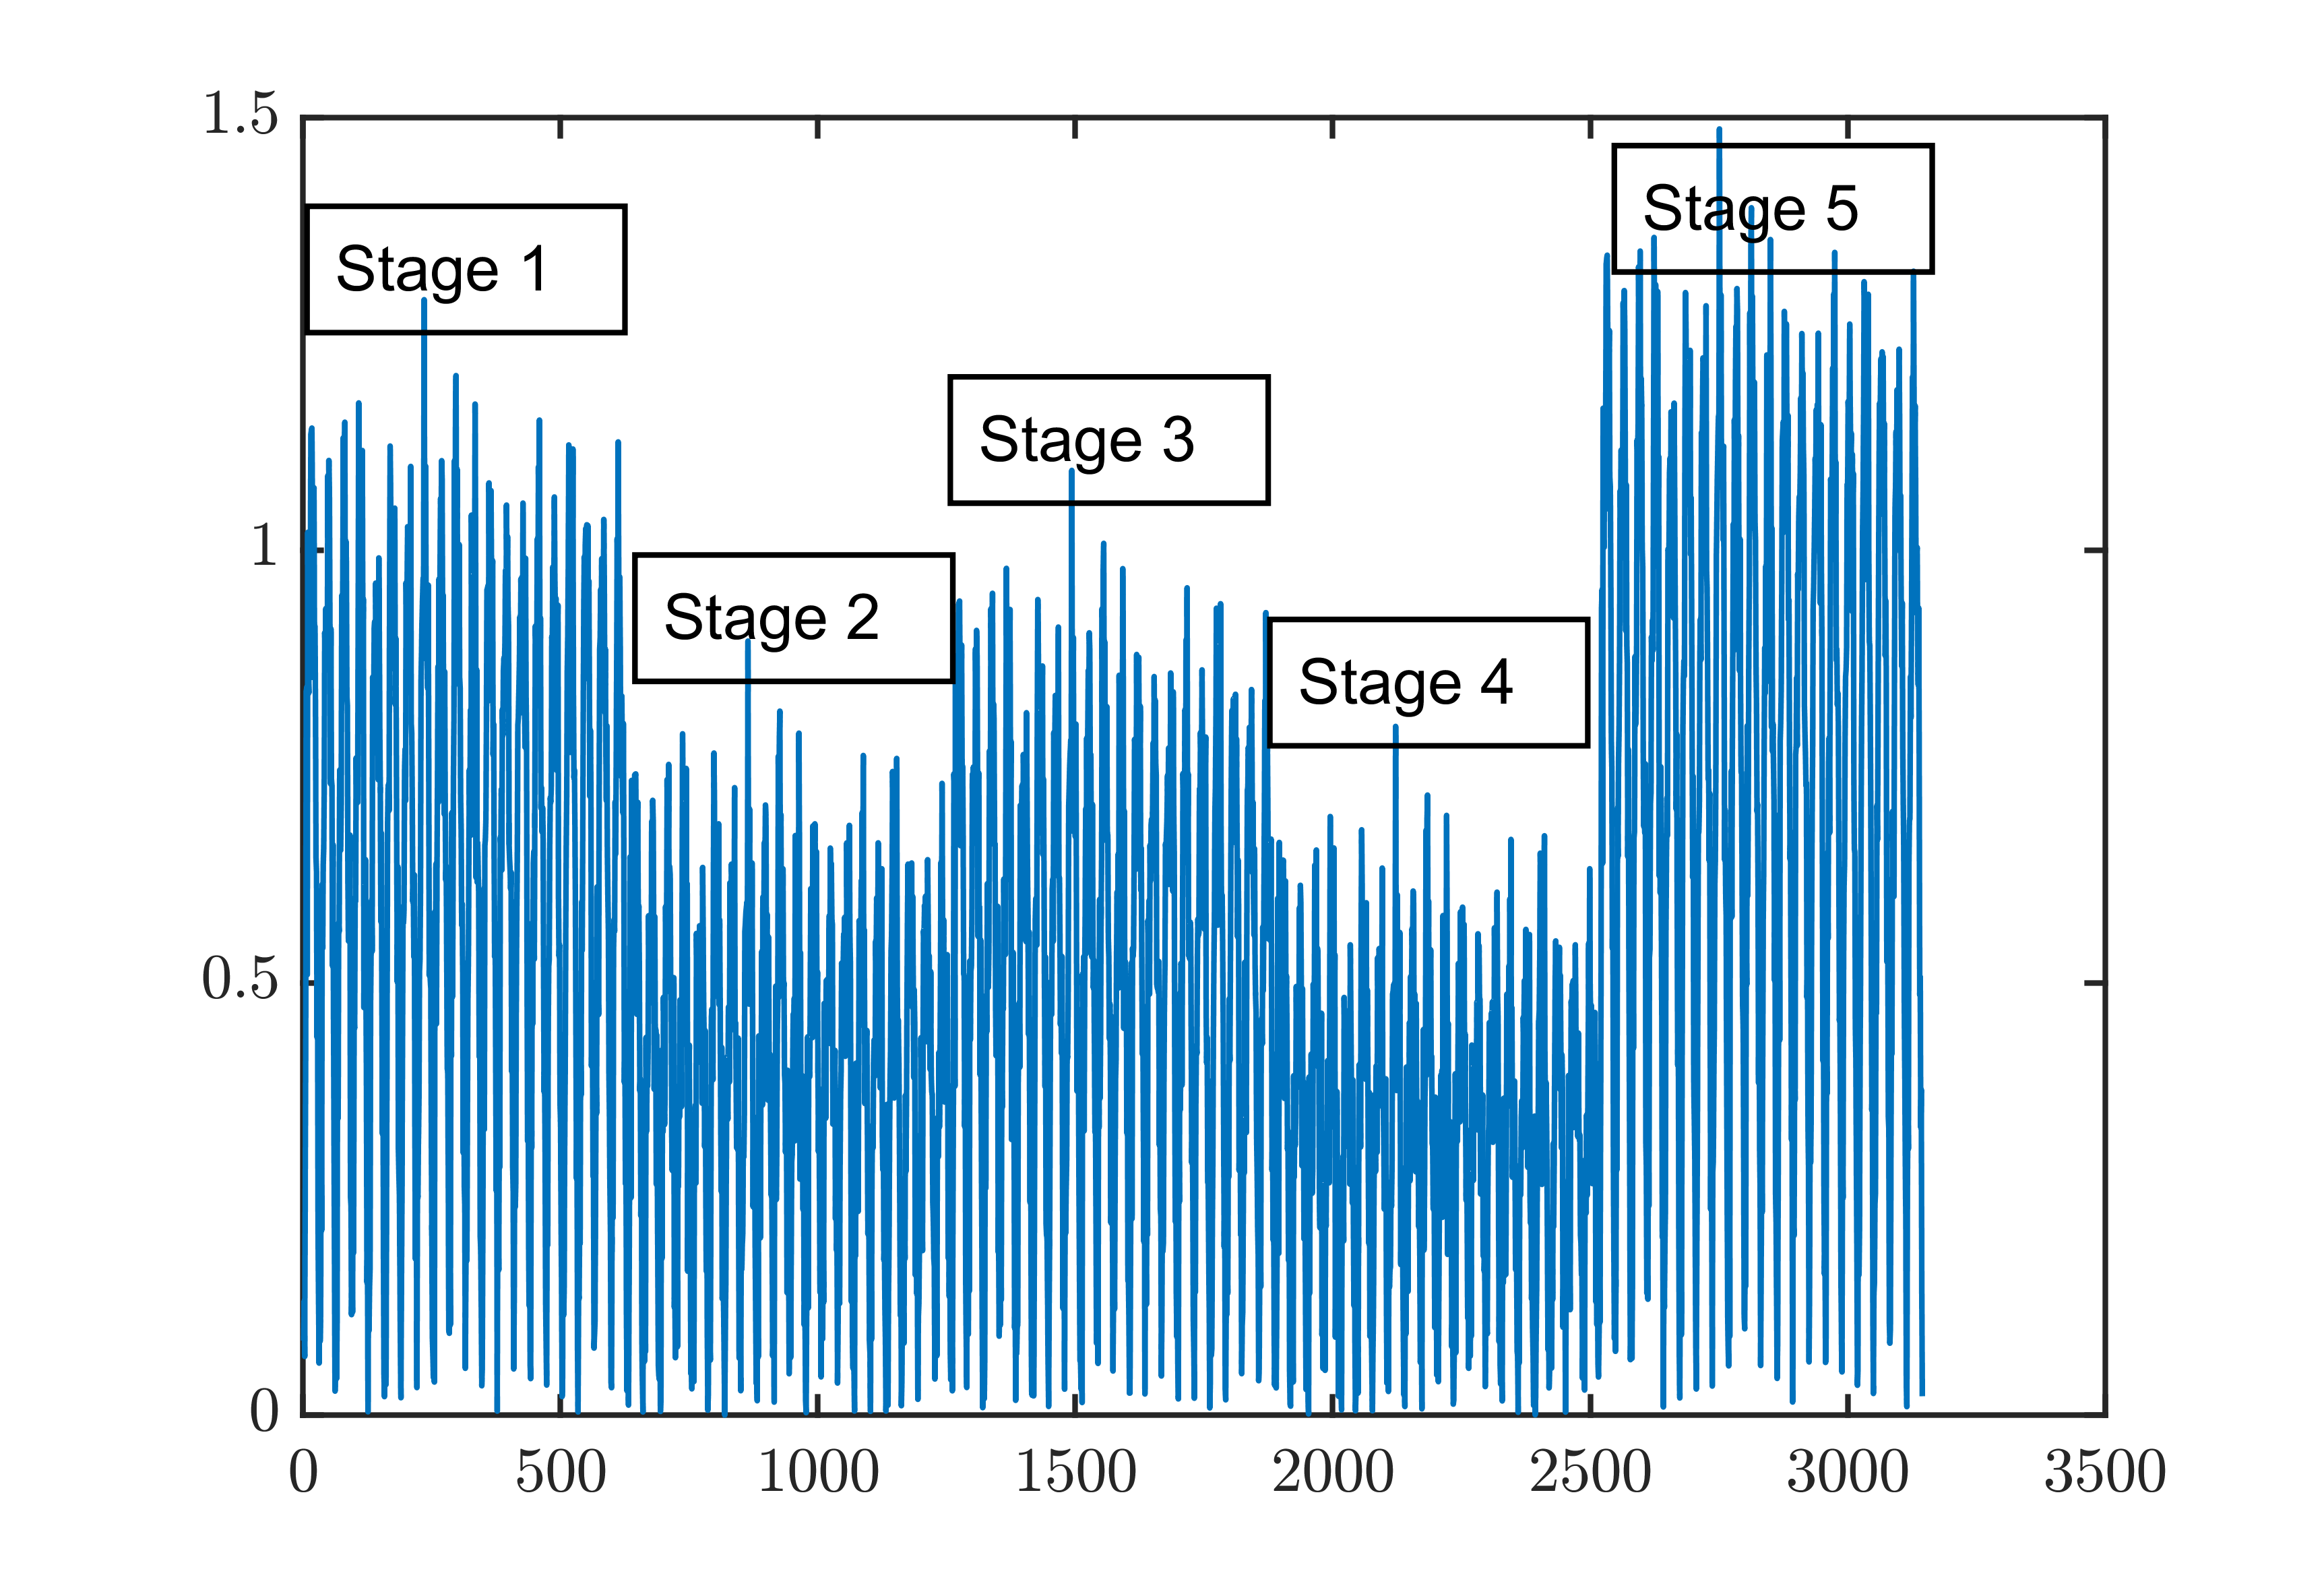
\includegraphics[scale = 0.7]{figures/ch1/amplitude.png}
\caption{Amplitude changes at the input of the PA \citep{guo2015}}
\label{fig:mem_amp}
\end{figure}




In modern communication systems, the input power to the PA may be adjusted corresponding to the needs by the network. This makes a suddenly increase or decrease in the power as depicted in figure \ref{fig:mem_amp} which makes the PA work in the transient stage. The stages of the PA can be divided into two stages, where, 1) Transient stage: The period when the input power of the PA jumps from one level
to another and 2) the steady-state stage: the period when the
average input power level is fixed \citep{guo2015}. In \citep{liu2007} memory effects is defined as following:  
\textit{Memory effects
can generally be classified as electro-thermal memory effects
and electrical memory effects. The electro-thermal memory
effects are mainly caused by the thermal capacitance and
resistance that form a low pass thermal filter. The electrical
memory effects can be mainly attributed to the non-constant
frequency response of the PA around the carrier frequency,
the impedance variation of bias circuits at baseband, and the
harmonic loading in the PA power stage.} Even modelling of this is rather comprehensive the DPD still needs to take these effects into account to generate a non-distorted output at the PA.  

\section{AM/AM and AM/PM distortion}
If the input signal to the PA is modelled as equation \ref{eq:amam1}

\begin{equation}\label{eq:amam1}
x(t) = a(t)e^{j\phi(t)}
\end{equation}

Where $a(t)$ is the envelope of the signal and $e^{j\phi(t)}$ is the phase of the input signal. Then the distorted output of the amplifier will be that of equation \ref{eq:amam1} where $g()$ is the amplitude distortion and $f()$ is the phase distortion also called Amplitude to Amplitude (AM/AM) and Amplitude to Phase (AM/PM) distortion. AM/AM distortion can be defined as the deviation from the constant gain when PA is
operated in compression region. On the other hand, the increased phase change at compression
region can be termed as AM/PM distortion.In presence of wideband signals having non constant amplitude, PA behaves as nonlinear system and exhibits two types of nonlinearities which is static distortion and memory effects.  

\begin{equation}\label{eq:amam2}
y(t) = g(a(t))e^{j\phi(t)+f(a(t))}
\end{equation}


\section{Crosstalk}
Crosstalk is coupling from one branch to another branch. When only a signal is present on a single branch, no crosstalk would appear to this branch. On the other hand if a signal is presented at two branches then crosstalk would appear to both of them. There exist three types of crosstalk where 1) Crosstalk before the PA's, see figure \ref{fig:cross_bf}, 2) Crosstalk after the PA's, see figure \ref{fig:cross_af}. 3) Crosstalk on the antennas and mishmash due to coupling. Crosstalk before the PA is also called nonlinear since it is amplified by the non linear PA. The nonlinear crosstalk and the PA nonlinear response should be jointly
compensated by a predistorter to get a reliable system performance \citep{islam2017} denoted $\mu_k (.)$. The output from the branches would become that of equation \ref{eq:nonlin}.

\begin{equation} \label{eq:nonlin}
Y_{1k} = fk(uk(X_{11},X_{12},X_{13},X_{1k}))
\end{equation}   

Where X is the input signal, Y is the output and $fk$ is the PA response. 

\begin{figure}[H]
  \centering
  \begin{minipage}[b]{0.5\textwidth}
	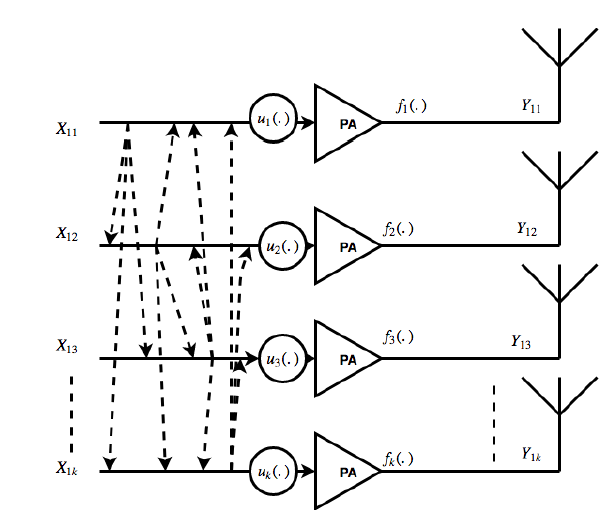
\includegraphics[scale = 0.5]{figures/ch1/crosstalk_before}
	\caption{Crosstalk before PA \citep{islam2017}}	
    \label{fig:cross_bf}
  \end{minipage}
  \hfill
  \begin{minipage}[b]{0.4\textwidth}
	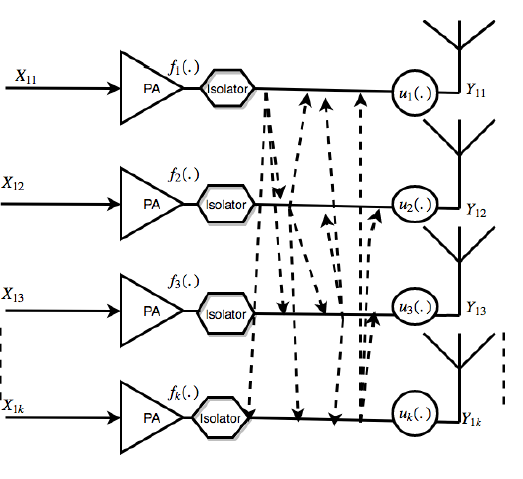
\includegraphics[scale = 0.5]{figures/ch1/crosstalk_after}
	\caption{Crosstalk after PA \citep{islam2017}}
    \label{fig:cross_af}
  \end{minipage}
\end{figure}

Crosstalk after the PA is called linear since it has an linear impact. In figure \ref{fig:cross_af} the output of the amplifier is connected to an isolator, which makes the output unaffected by reflections. A linear model can therefore be used which is shown in equation \ref{eq:lin_iso}. 

\begin{equation} \label{eq:lin_iso}
Y_{1k} = \mu_k(f1(X_{11}),f2(X_{12}),f3(X_{13})..fk(X_{1k}))
\end{equation}     

When no isolators is presented the output will now be affected by the crosstalk or mutual-coupling between the antennas. A sketch of this is depicted in figure \ref{fig:cross_ant} where $a_{1k}$ is the incoming signal to the amplifier, $b_{2k}$ is the output from the amplifier and $a_{2k}$ is the reflected signal form the antenna array at the k'th branch \citep{Hausmair2017}. The relation between $a_{2k}$
and the output signals $b_{2k}$ is determined by the characteristics
of the antenna array. The system model of the multi-antenna
transmitter can, therefore, be split in to a crosstalk and
mismatch model (CTMM). This block can further be used together with a dual-input-DPD which holds the model for the PA, see figure \ref{fig:cross_ctmm}. 


\begin{figure}[H]
  \centering
  \begin{minipage}[b]{0.5\textwidth}
	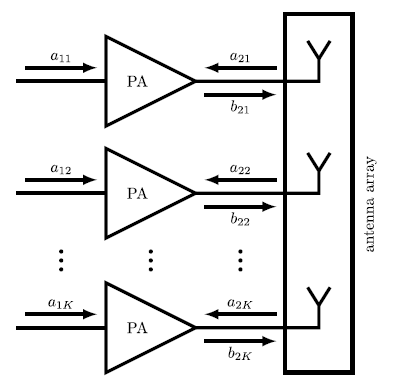
\includegraphics[scale = 0.5]{figures/ch1/crosstalk_antenna}
	\caption{Model of the antenna crosstalk \citep{Hausmair2017}}	
    \label{fig:cross_ant}
  \end{minipage}
  \hfill
  \begin{minipage}[b]{0.4\textwidth}
	\includegraphics[scale = 0.5]{figures/ch1/crosstalk_ctmm.png}
	\caption{The predistortion method consists of two main blocks: one linear CTMM block
for the whole transmitter and a dual-input DPD block in every transmit path. \citep{Hausmair2017}}
	\label{fig:cross_ctmm}
  \end{minipage}
\end{figure}


\section{Antenna Diversity and MIMO}

\begin{figure}[H]
\centering 
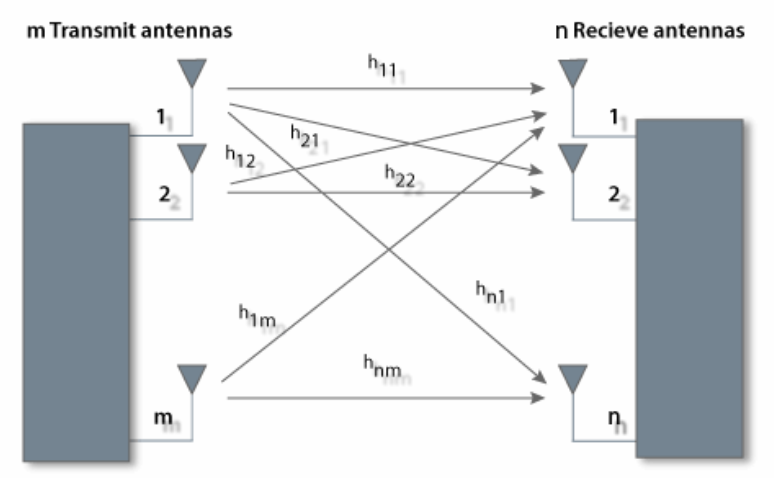
\includegraphics[scale = 0.4]{figures/ch1/mimo.png}
\caption{Concept of mimo}
\label{fig:mimo}
\end{figure}

MIMO (Multiple Input Multiple Output) systems are systems with Multiple Element Antennas at both link ends. The antenna elements of a MIMO system can be used for four different purposes: beamforming, diversity, interference suppression, and spatial multiplexing which is transmission of several data streams in parallel that allows improvement of capacity. A MIMO system is modelled as in equation \ref{eq:mimo} and is also depicted in figure \ref{fig:mimo}.

\begin{equation}\label{eq:mimo}
\textbf{y = Hx+n}
\end{equation}  

Where \textbf{y} is the received vector, \textbf{H} is the channel matrix, \textbf{x} is the transmitted vector and \textbf{n} is noise. If the full channel matrix is known then the transmitted vector can be obtained by the receiver like equation \ref{eq:mimo2}.  

\begin{equation}\label{eq:mimo2}
\textbf{x+n} = \textbf{H}^{1} \textbf{y}
\end{equation}  

The principle of MIMO is to ensure that the same information reaches the receiver on several
statistically independent channels. In MIMO systems, several transmits paths is archived by use of several antennas, which gives a spatial separation if they are separated enough to give a correlation factor $\rho$ that is below $0.5 - 0.7$ \citep{molisch2011}. The formula for the envelope correlation factor between two antennas is given by equation \ref{eq:corr_fac}. The formula assumes that the WSSUS (Wide-Sense Stationary Uncorrelated Scattering) model is valid, no LOS exists, the power delay profile has an exponential shape, the incident power is isotropically distributed in azimuth and only propagates in the horizontal plane, and an omni-antenna is used.

\begin{eqnarray} \label{eq:corr_fac}
\rho = \frac{J_0^2( k_0 v \tau)}{1+(2\pi)^2 S_\tau^2(f_2 - f_1)^2 }
\end{eqnarray}      

Where $J_0$ is the Bessel function of the first kind and $S_\tau$ is the delay-spread of the channels. If the correlation between two antennas is investigated for the same frequency, then the formula can be rewritten as equation \ref{eq:corr_fac_re} because $f2-f1=0$.

\begin{eqnarray} \label{eq:corr_fac_re}
\rho = J_0^2( 2\pi d)^{-1}
\end{eqnarray} 

Where $d$ is the element spacing given in wavelengths. A plot of this can bee seen in figure \ref{fig:correlation}.

\begin{figure}[H]
\centering 
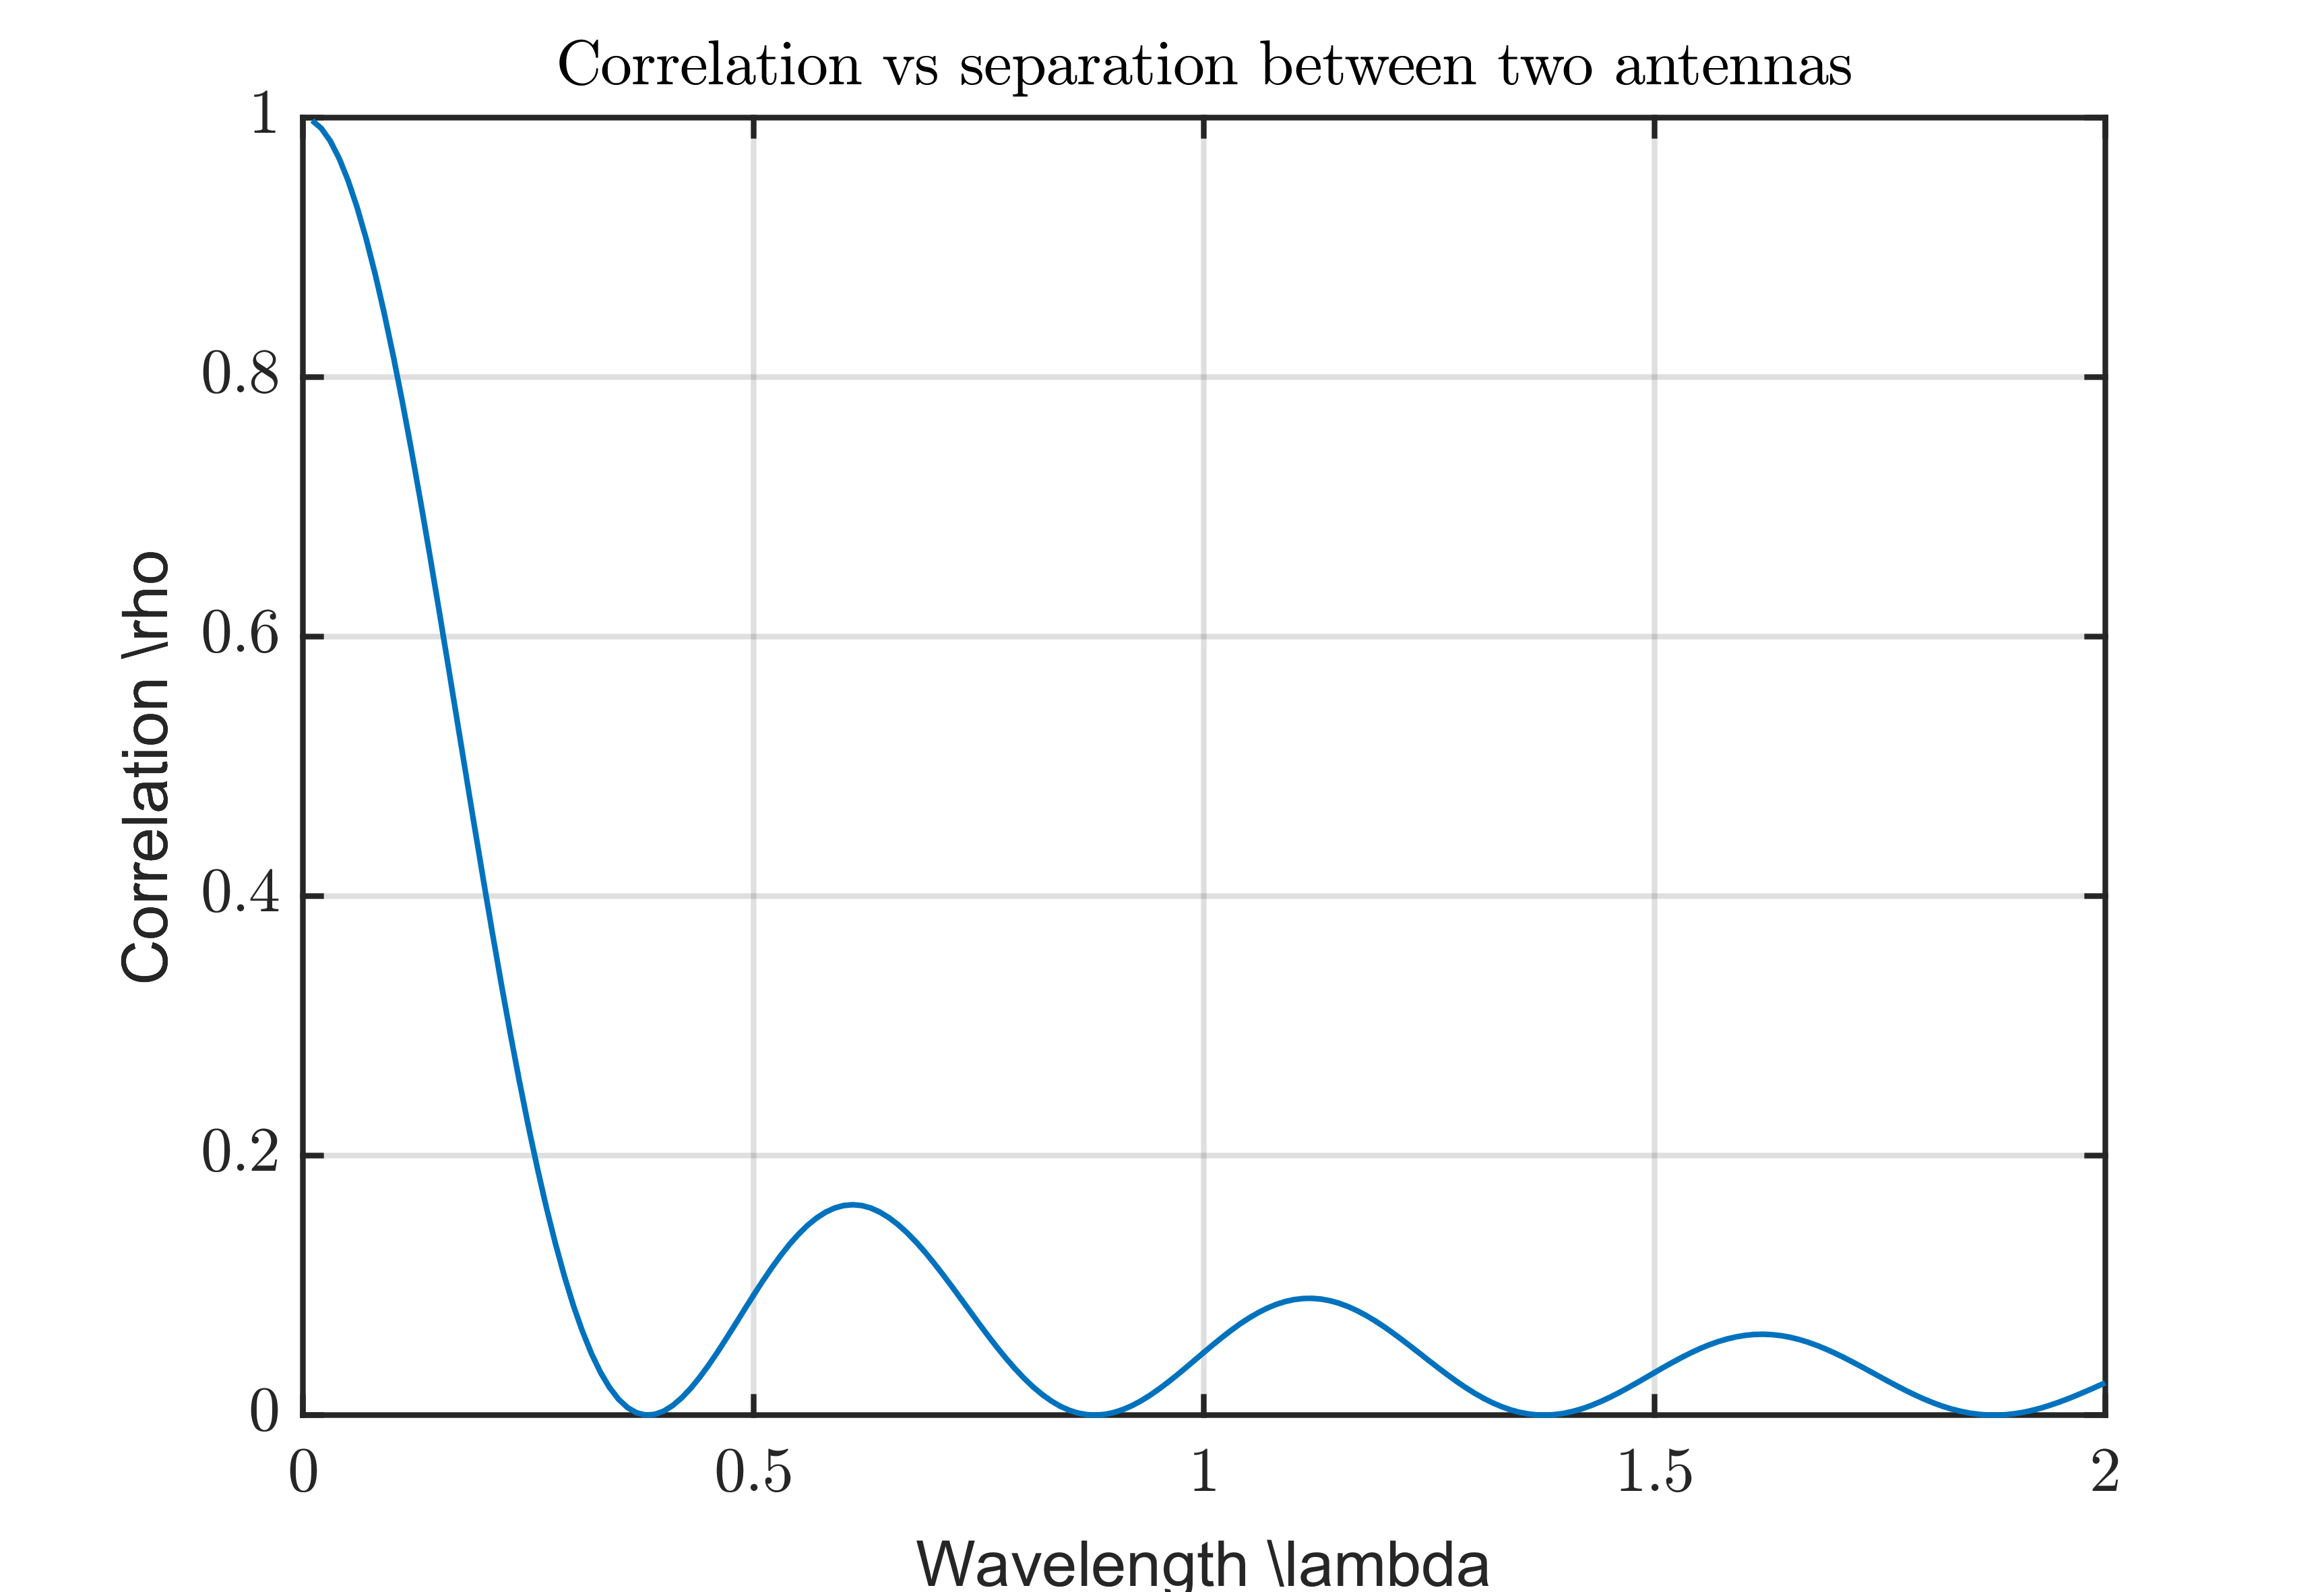
\includegraphics[scale = 0.7]{figures/ch1/correlation.png}
\caption{Correlation factor for two antennas versus distance}
\label{fig:correlation}
\end{figure}

Another method to calculate the correlation factor is to use measured or simulated S-parameters as shown in equation \ref{eq:spar_corr} \citep{wang2011} where k is the propagation constant and d the distance in meters. 

\begin{equation} \label{eq:spar_corr}
\rho = \frac{A+B J_0(kd)}{B+A J_0(kd)}
\end{equation}

\begin{equation} 
A = -2Re(S_{12}^*(1-S_{11}))
\end{equation}

\begin{equation} 
B = |1-S_{11}|^2 + |S_{12}|^2
\end{equation}

A simulation has been made in CST studio with 4 antennas separated $0.1\lambda$ at $f = 3.5Ghz$ or 8.6mm, see figure \ref{fig:correlation}. The simulated S-parameters has been imported to MATLAB and the formula is used to generate the correlation plot in figure \ref{fig:correlation_plot}. From the figure it can bee seen that when the frequency increases the correlation becomes lower. 


\begin{figure}[H]
\centering 
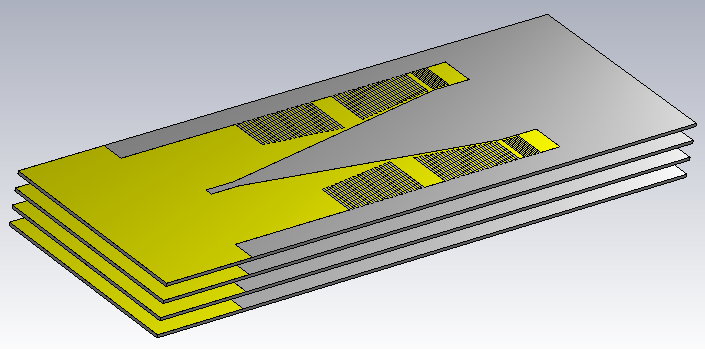
\includegraphics[scale = 0.7]{figures/ch1/antenna_array.png}
\caption{4 wideband PCB antennas separated 8.6mm }
\label{fig:correlation}
\end{figure}

\begin{figure}[H]
\centering 
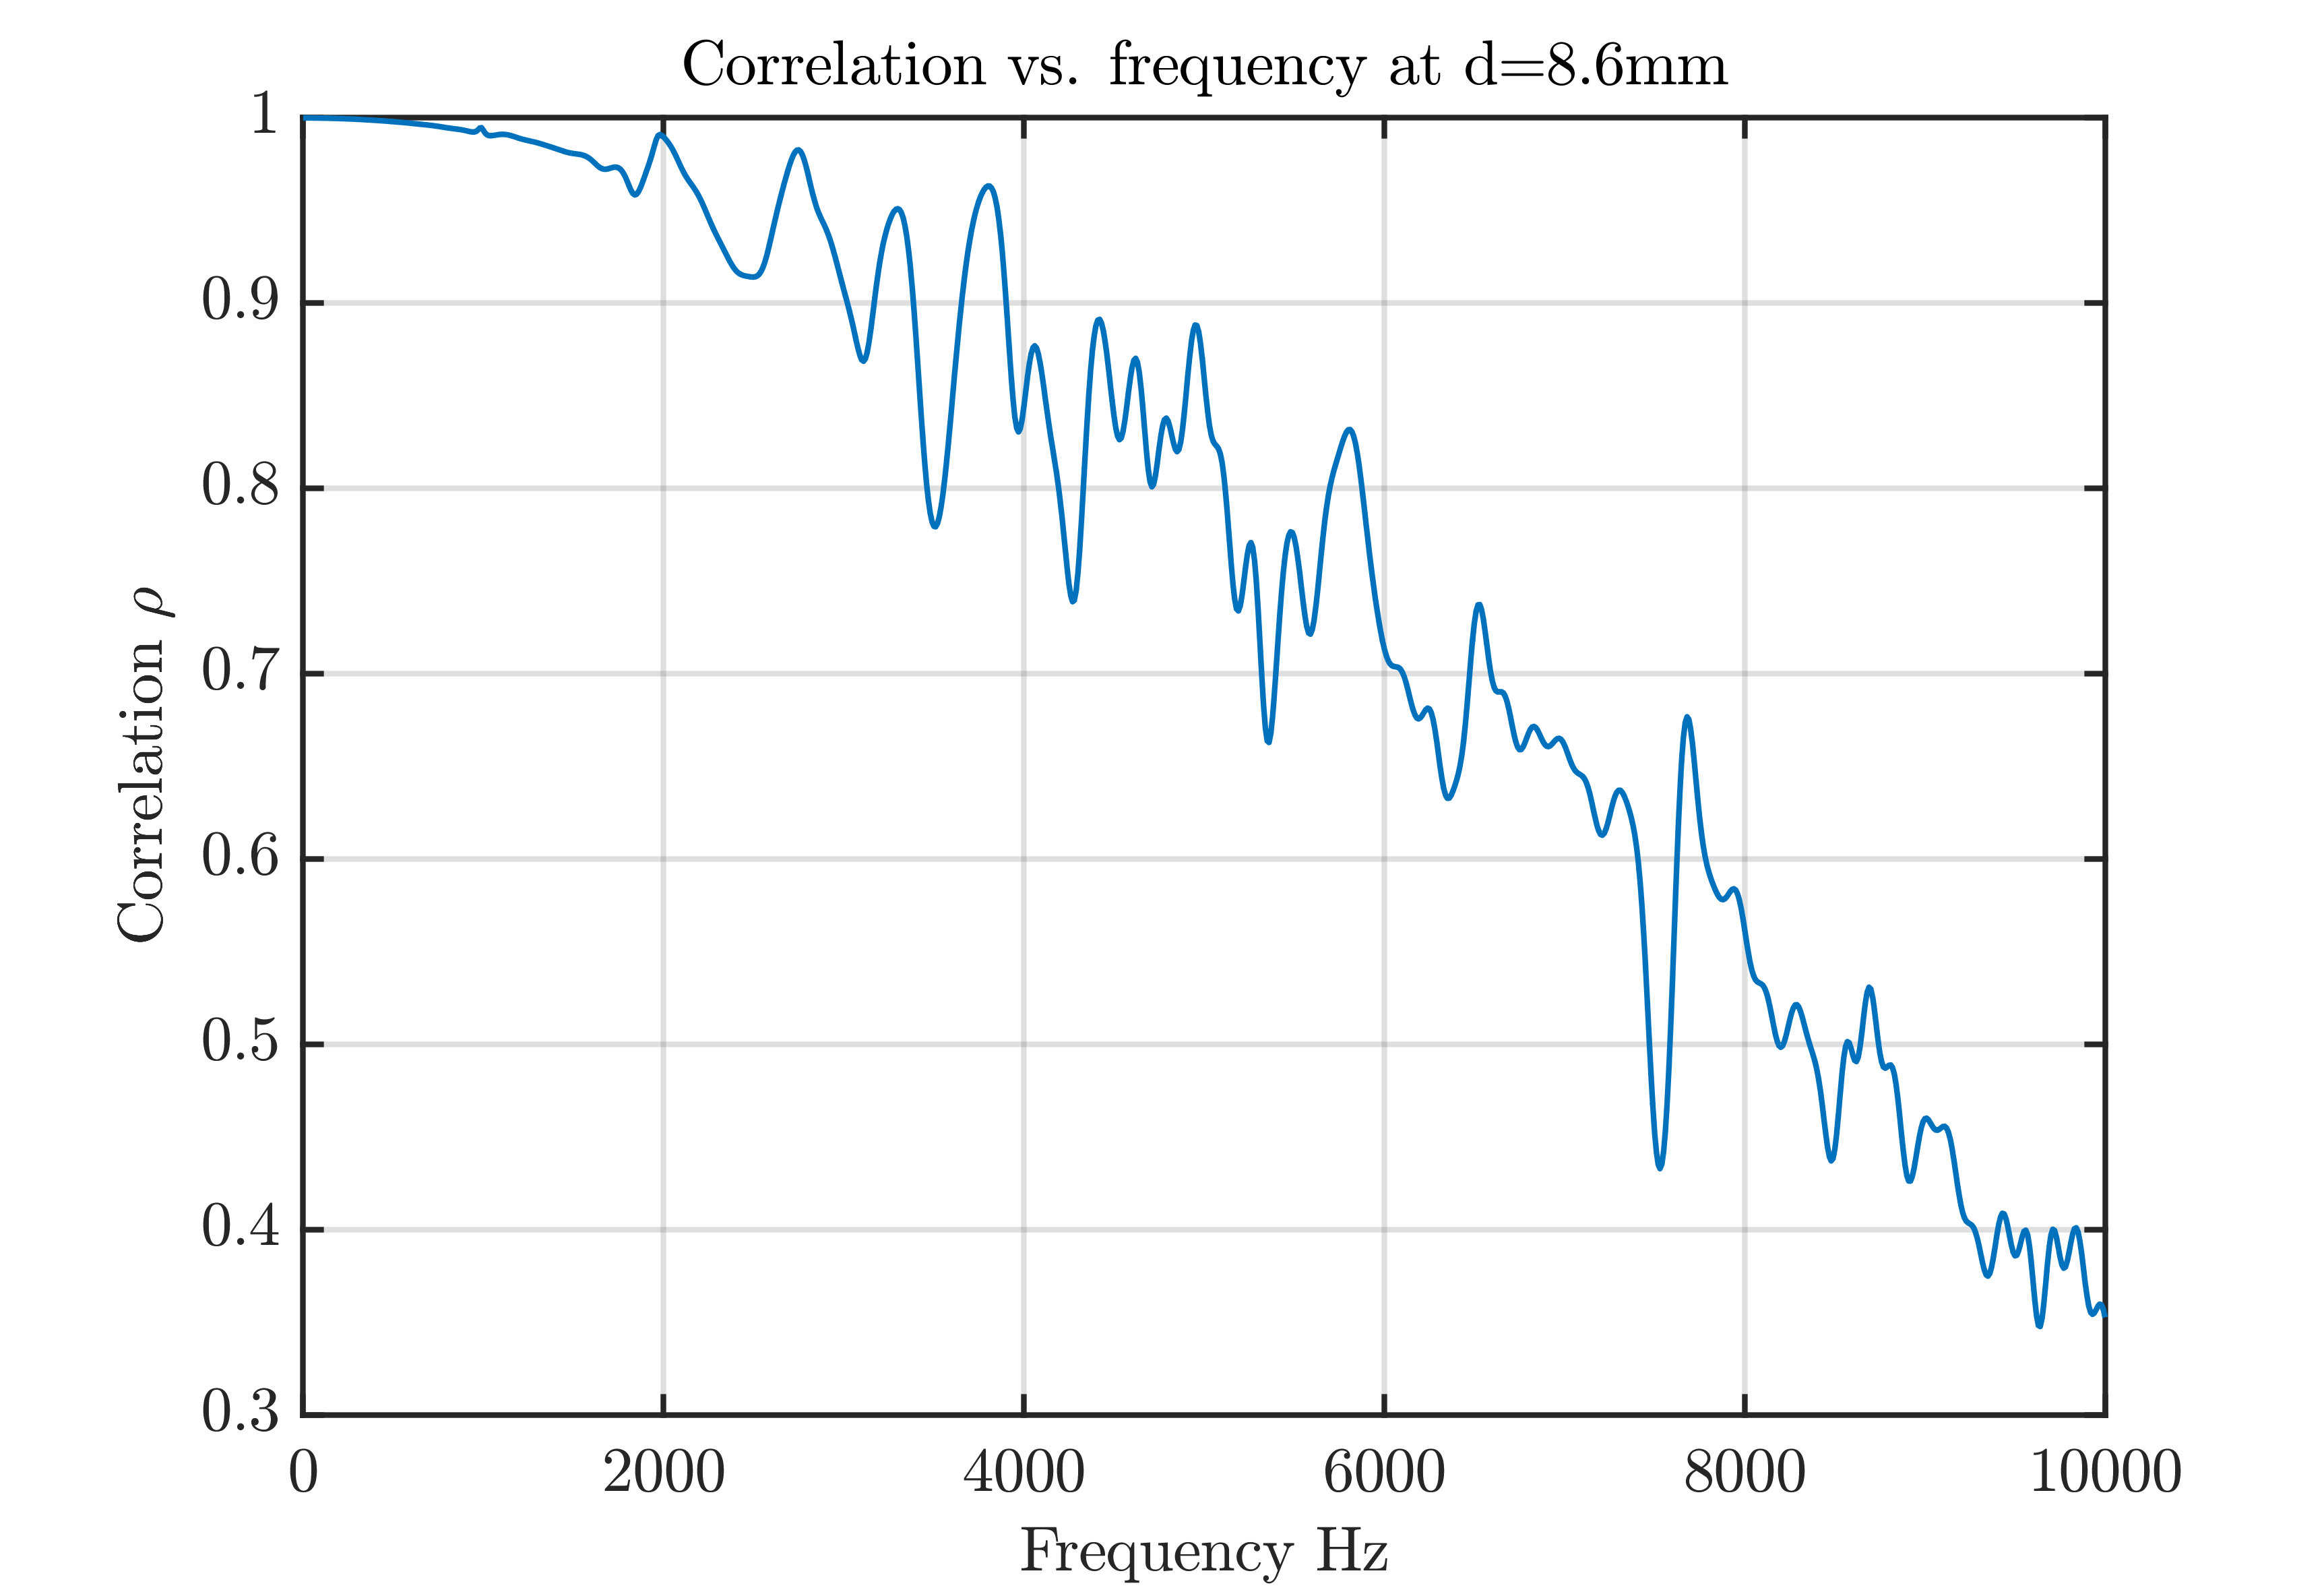
\includegraphics[scale = 0.9]{figures/ch1/antenna_array_corr.png}
\caption{Correlation between antenna 1 and 2}
\label{fig:correlation_plot}
\end{figure}




